%!TeX program = pdflatex
% LaTeX Template
% Author: Geoff Boeing
% Web: https://geoffboeing.com/
% Repo: https://github.com/gboeing/latex-template
% Some considerations:
% - use pdflatex instead of xelatex/lualatex for compatibility with arxiv and publishers
% - use natbib/bibtex instead of biblatex/biber for compatibility with arxiv and publishers
% - avoid system fonts, instead use self-contained ebgaramond/tgheros font packages
% - avoid importing other packages unless truly necessary (it rarely is)
% - compile often, check log for any warnings/errors, and resolve them promptly when they arise

\newcommand{\myname}{Geoff Boeing}
\newcommand{\myemail}{boeing@usc.edu}
\newcommand{\myaffiliation}{Department of Urban Planning and Spatial Analysis\\Sol Price School of Public Policy\\University of Southern California}
\newcommand{\paperdate}{April 2024}
\newcommand{\papertitle}{This Is My Paper Title}
\newcommand{\papercitation}{Boeing, G. 2024. \papertitle. Under review at \emph{Journal Name}.}
\newcommand{\paperkeywords}{Urban Planning, Transportation, Data Science}

\RequirePackage[l2tabu,orthodox]{nag} % warn if using any obsolete or outdated commands
\documentclass[12pt,letterpaper]{article} % document style

% import encoding and font packages for pdflatex, in order
\usepackage[T1]{fontenc} % output T1 font encoding (8-bit) so accented characters are a single glyph
\usepackage[utf8]{inputenc} % allow input of utf-8 encoded characters
\usepackage{ebgaramond} % document's serif font
\usepackage{tgheros} % document's sans serif font

% import language, regionalization, microtype, and setspace in order
\usepackage[strict,autostyle]{csquotes} % smart and nestable quote marks
\usepackage[USenglish]{babel} % automatically regionalize hyphens, quote marks, etc
\usepackage{microtype} % improves text appearance with kerning, etc
\usepackage{setspace} % configure spacing between lines

% import everything else
\usepackage{abstract} % allow full-page title/abstract in twocolumn mode
\usepackage{authblk} % footnote-style author/affiliation info
\usepackage{booktabs} % better looking tables
\usepackage{caption} % custom figure/table caption styles
\usepackage{datetime} % enable formatting of date output
\usepackage[final]{draftwatermark} % watermark paper as a draft
\usepackage{endnotes} % enable endnotes
\usepackage{geometry} % configure page dimensions and margins
\usepackage{graphicx} % better inclusion of graphics
\usepackage{hyperref} % hypertext in document
\usepackage{natbib} % author-year citations w/ bibtex, including textual and parenthetical
\usepackage{rotating} % rotate wide tables or figures on a page to make them landscape
\usepackage{titlesec} % custom section and subsection heading
\usepackage{url} % make nice line-breakble urls

% print only the month and year when using \today
\newdateformat{monthyeardate}{\monthname[\THEMONTH] \THEYEAR}

% location of figure files, via graphicx package
\graphicspath{{./figures/}}

% configure the page layout, via geometry package
\geometry{
    paper=letterpaper, % paper size
    top=3.8cm, % margin sizes
    bottom=3.8cm,
    left=4cm,
    right=4cm}
\setstretch{1} % line spacing
\clubpenalty=10000 % prevent orphans
\widowpenalty=10000 % prevent widows

% set section/subsection headings as the sans serif font, via titlesec package
\titleformat{\section}{\normalfont\sffamily\large\bfseries\color{black}}{\thesection.}{0.3em}{}
\titleformat{\subsection}{\normalfont\sffamily\small\bfseries\color{black}}{\thesubsection.}{0.3em}{}

% make figure/table captions sans-serif small font
\captionsetup{font={footnotesize,sf},labelfont=bf,labelsep=period}

% configure pdf metadata and link handling, via hyperref package
\hypersetup{
    pdfauthor={\myname},
    pdftitle={\papertitle},
    pdfsubject={\papertitle},
    pdfkeywords={\paperkeywords},
    pdffitwindow=true, % window fit to page when opened
    breaklinks=true, % break links that overflow horizontally
    colorlinks=false, % remove link color
    pdfborder={0 0 0} % remove link border
}

\begin{document}

\title{\papertitle\footnote{{Preprint of: \papercitation}}}
\author[]{\myname\footnote{Email: \href{mailto:\myemail}{\myemail}}}
\affil[]{\myaffiliation}
\date{\paperdate}

\maketitle

\begin{abstract}
Nunc efficitur dui non elementum tincidunt. Sed eget ultricies dui, nec congue massa. Fusce at faucibus arcu, a dapibus leo. Donec congue viverra lorem, et viverra massa pellentesque eu. Mauris dictum efficitur lectus, nec tempus velit viverra at. Pellentesque habitant morbi tristique senectus et netus et malesuada fames ac turpis egestas. In tristique urna purus, a viverra sapien vehicula at. Donec id lectus dui. Class aptent taciti sociosqu ad litora torquent per conubia nostra, per inceptos himenaeos. Ut viverra leo ac velit aliquam, id pellentesque est maximus. Proin laoreet aliquet ex vel semper. Integer congue sollicitudin elit, ut tincidunt odio tincidunt quis. Duis eu mi sed massa pellentesque efficitur.
\vspace{1cm}
\end{abstract}


\section{Introduction}

Lorem ipsum\endnote{This is my note.} dolor sit amet, \emph{consectetur} adipiscing elit. Mauris fermentum sapien at libero finibus, lacinia tincidunt mi varius. \enquote{Vestibulum eget pretium urna.} Phasellus consectetur sem eu egestas scelerisque. Etiam tempor porttitor nulla, et rhoncus dui. Praesent iaculis sollicitudin augue et luctus. Quisque congue odio a suscipit sodales. Nullam mattis, ligula at vulputate lacinia, est nisi faucibus felis, ac gravida orci ligula sit amet nulla. Sed commodo magna semper interdum facilisis. Proin porttitor tortor a purus convallis malesuada \citep{boeing_off_2021}. Ut tempus eleifend eros, lacinia lobortis urna rhoncus ut. Donec in sapien tincidunt, consectetur velit ut, posuere nibh. Cras finibus imperdiet sem nec placerat. Donec efficitur metus eu sapien semper elementum. Nullam eros dui, rhoncus lacinia libero ac, pretium pellentesque justo. In a laoreet mauris, ac sollicitudin erat. Phasellus mattis tincidunt diam id sagittis.

Nullam consequat ex lectus. Aliquam sagittis lacus quis dui tincidunt, eget accumsan dolor dictum. Duis vel ultricies sem. Aliquam dapibus tellus consequat, ornare diam vitae, dapibus dui. Maecenas blandit posuere augue quis ornare. Fusce posuere tortor fringilla lacus viverra, a iaculis quam vehicula. Aenean convallis tellus ut leo egestas, ac consequat nisi efficitur.

\section{Background}

Nunc porttitor pretium eleifend \citep{boarnet_travel_2001}. In hendrerit dolor leo, at rutrum erat finibus ac. Aliquam id nisi ipsum. In tristique, neque nec condimentum consectetur, neque nisi imperdiet nibh, at pellentesque urna quam non leo. Orci varius natoque penatibus et magnis dis parturient montes, nascetur ridiculus mus. Ut sed consequat nunc, sit amet iaculis augue. Mauris in blandit erat, non dapibus nulla. Duis condimentum pretium felis, vel commodo justo luctus non. Integer consectetur, ipsum consectetur tristique pharetra, ligula purus ultricies diam, et lacinia odio sapien et arcu. Morbi vel semper urna, in consectetur massa. Mauris rutrum sem nec tortor tincidunt porta. Mauris maximus vehicula nisi, id cursus leo laoreet ac. Pellentesque habitant morbi tristique senectus et netus et malesuada fames ac turpis egestas. Maecenas a lacus vel nisl volutpat vehicula.

\section{Methods}

In hendrerit dolor leo, at rutrum erat finibus ac. Aliquam id nisi ipsum. In tristique, neque nec condimentum consectetur, neque nisi imperdiet nibh, at pellentesque urna quam non leo. Orci varius natoque penatibus et magnis dis parturient montes, nascetur ridiculus mus. Ut sed consequat nunc, sit amet iaculis augue. Mauris in blandit erat, non dapibus nulla. Duis condimentum pretium felis, vel commodo justo luctus non. Integer consectetur, ipsum consectetur tristique pharetra, ligula purus ultricies diam, et lacinia odio sapien et arcu. Morbi vel semper urna, in consectetur massa. Mauris rutrum sem nec tortor tincidunt porta. Mauris maximus vehicula nisi, id cursus leo laoreet ac. Pellentesque habitant morbi tristique senectus et netus et malesuada fames ac turpis egestas. Maecenas a lacus vel nisl volutpat vehicula.

\subsection{Data}

Nunc efficitur dui non elementum tincidunt. Sed eget ultricies dui, nec congue massa. Fusce at faucibus arcu, a dapibus leo. Donec congue viverra lorem, et viverra massa pellentesque eu. Mauris dictum efficitur lectus, nec tempus velit viverra at. Pellentesque habitant morbi tristique senectus et netus et malesuada fames ac turpis egestas. In tristique urna purus, a viverra sapien vehicula at. Donec id lectus dui. Class aptent taciti sociosqu ad litora torquent per conubia nostra, per inceptos himenaeos. Ut viverra leo ac velit aliquam, id pellentesque est maximus. Proin laoreet aliquet ex vel semper.

\begin{equation}
    \label{eq:my_equation}
    D_t = \frac{R_t + I_t - O_t}{A_t}
\end{equation}

Integer congue sollicitudin elit, ut tincidunt odio tincidunt quis. Duis eu mi sed massa pellentesque efficitur. Suspendisse fringilla dolor sed erat finibus consequat. Integer in metus vel odio hendrerit efficitur. Nulla sed orci nec mi commodo ultricies mattis non tortor.

\subsection{Analysis}

Quisque faucibus varius elit eu accumsan. Vivamus sit amet arcu at nibh auctor vulputate. Suspendisse dolor est, lacinia quis justo sodales, varius rhoncus nisi. Nulla maximus urna pulvinar dui pellentesque ultrices. Sed tincidunt consectetur massa, tincidunt sollicitudin odio eleifend in. Cras ornare ante non semper efficitur. Morbi vel maximus nisi, ac luctus sapien. Etiam augue nisi, aliquam vel quam quis, dignissim dignissim orci. Phasellus ultricies purus in ante scelerisque pulvinar. Morbi faucibus fringilla congue. Aenean accumsan est sit amet dolor maximus, vel posuere quam semper. Sed vehicula cursus gravida. Pellentesque auctor in elit ut laoreet. Proin iaculis condimentum turpis. Aenean egestas semper laoreet. Ut ornare dui quis lacus feugiat, eget posuere odio rutrum.

\section{Findings}

Integer urna mauris, varius at vestibulum id, elementum id purus. Vestibulum tincidunt, odio at tempor tempor, ex eros iaculis quam, aliquet blandit felis lectus sit amet diam. Morbi vel sapien at mi rhoncus molestie. Sed nec laoreet tortor. Nunc id dui fringilla, laoreet velit quis, venenatis ipsum. Phasellus semper mauris in diam ultrices, vitae tincidunt nisi euismod. Pellentesque quis lacinia lectus. Morbi nec dolor a ipsum bibendum viverra in nec lacus. Proin maximus sem vel bibendum dapibus. Quisque fringilla at ex at aliquet. Sed est quam, porta ac elit et, consectetur vestibulum leo. Integer nec quam a metus eleifend tempus. Vestibulum non varius arcu.

\subsection{Finding One}

 In posuere egestas lacus a hendrerit. Sed semper interdum lacus, non imperdiet ipsum faucibus nec Figure~\ref{fig:my_figure}. Cras a mollis purus. Morbi ut ornare neque. Praesent gravida velit nec lectus faucibus, nec vestibulum mi pharetra. Nulla molestie ultrices nisi, eget posuere velit feugiat vel. Duis fringilla felis libero, eget cursus felis consequat et. Donec sodales elit diam, ut faucibus lacus hendrerit et. Curabitur auctor finibus nisl, in rutrum purus imperdiet sit amet.

\begin{figure*}[tbp]
    \centering
    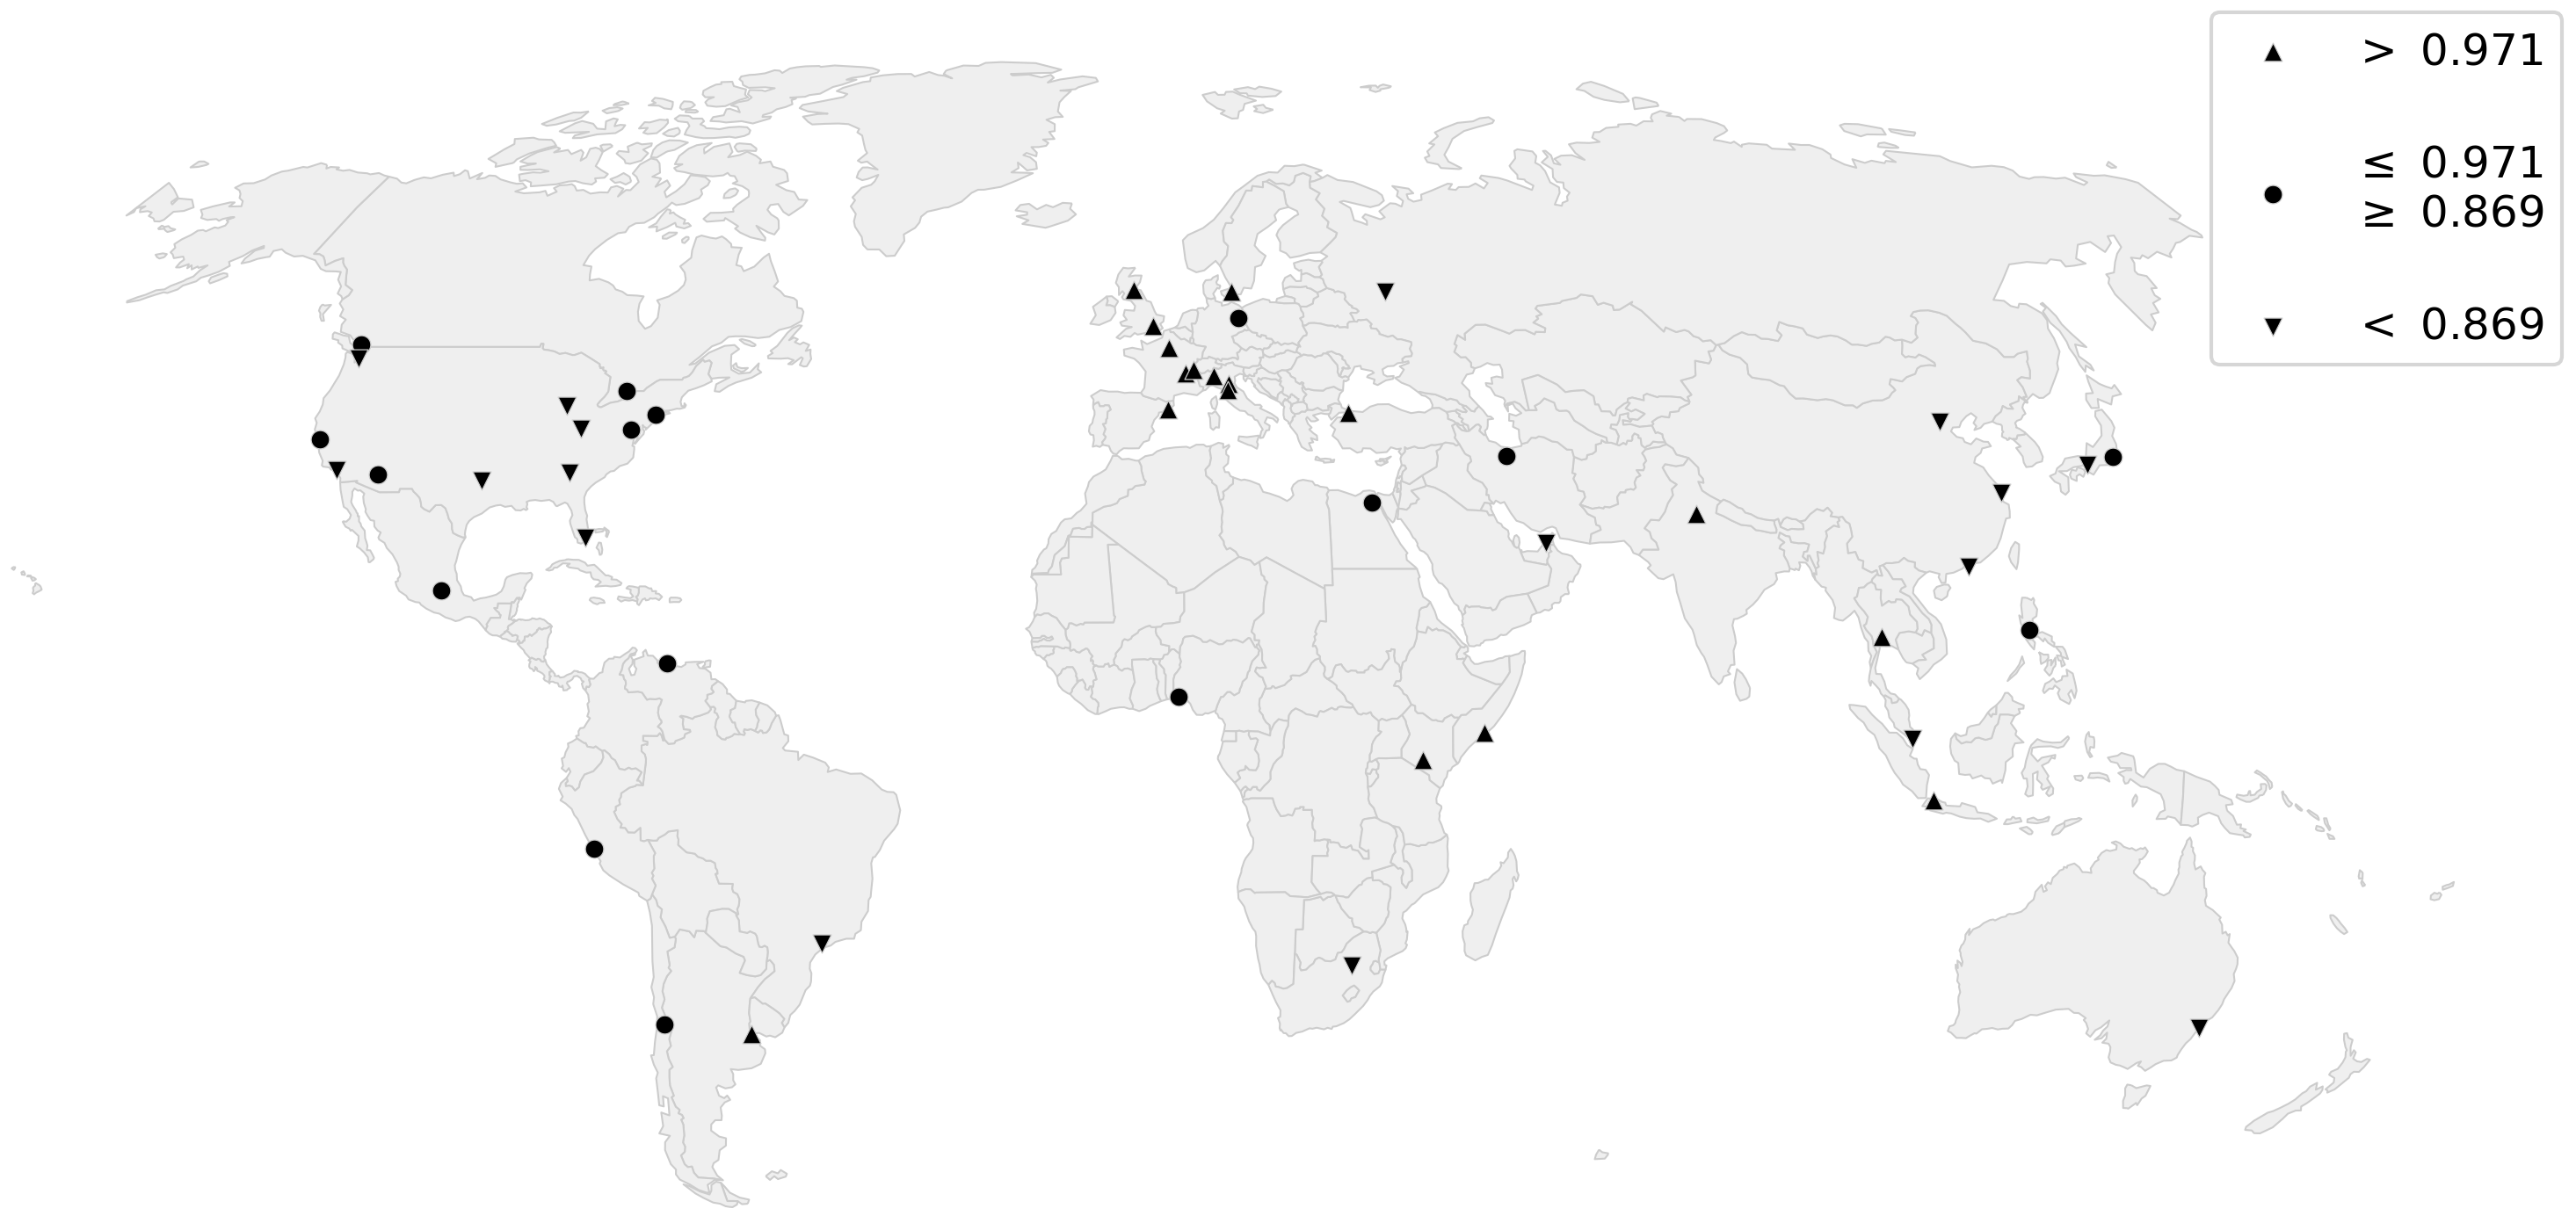
\includegraphics[width=0.95\textwidth]{example.png}
    \caption{This is the caption of my figure.}\label{fig:my_figure}
\end{figure*}

Pellentesque molestie pretium neque, eget laoreet ex. Curabitur quis lectus id neque tincidunt ullamcorper nec vel odio. Pellentesque tempus metus quam, non pellentesque nibh tempus et. Ut leo massa, iaculis nec lectus et, porttitor molestie eros. Vivamus eleifend dignissim purus, a egestas nisi iaculis ut. Maecenas interdum eros in orci aliquet pulvinar at nec lorem. Mauris et quam vel urna iaculis vulputate et sit amet velit. Curabitur massa nibh, viverra ornare gravida in, sodales nec ex. Fusce fermentum elementum nisi, ac porta magna tincidunt quis. Sed congue nunc eget mauris consequat gravida. Suspendisse fermentum risus sit amet auctor dapibus. Ut quam ex, finibus non imperdiet sit amet, semper ac erat. Vivamus convallis eget sapien ac pulvinar. Pellentesque ut pharetra lorem.

\subsection{Finding Two}

Proin eu ligula ut sem lacinia ullamcorper Table~\ref{tab:my_table}. Vivamus ullamcorper massa arcu, sed tincidunt dui dictum et. Vivamus finibus libero in leo semper, at fermentum ligula porta. Aliquam molestie ligula eget volutpat iaculis. Nam porttitor elit tortor, eget euismod risus mollis et. Mauris sit amet iaculis odio, eu fringilla leo. Phasellus pharetra vitae velit et faucibus. Mauris orci tellus, dignissim et quam eget, tincidunt pretium libero. In eu vehicula orci, vitae dignissim neque. In suscipit, risus eget lobortis dapibus, orci libero hendrerit lectus, a vulputate dui sem quis est. Suspendisse id tortor consequat ligula vehicula porta.

\begin{table*}[tbp]
    \centering
    \caption{This is the caption of my table.}\label{tab:my_table}
    \begin{tabular}{rrrr}
        \toprule
        Residential Pop &  Daytime Pop &  Land Area (km\textsuperscript{2}) &  Daytime Density \\
        \midrule
        1783  & 70728 & 0.556 & 127198 \\
        6172  & 42635 & 0.446 &  95652 \\
        2734  &  8006 & 0.092 &  86882 \\
        1500  &  4850 & 0.057 &  85743 \\
        4307  & 19051 & 0.240 &  79424 \\
        4233  & 22416 & 0.346 &  64768 \\
        3499  & 13051 & 0.214 &  60971 \\
        11502 & 92865 & 1.670 &  55617 \\
        3821  &  3319 & 0.061 &  54162 \\
        3073  &  4829 & 0.093 &  52122 \\
        \bottomrule
    \end{tabular}
\end{table*}

\section{Conclusion}

Aliquam pulvinar, augue id blandit scelerisque, orci nulla consequat purus, quis accumsan lectus leo eu tortor. Donec tempor dolor vel dui lobortis viverra. Nam at orci quam. Ut ut efficitur tellus, in rhoncus odio. Duis egestas tortor lectus, eget sollicitudin eros ornare ac. Suspendisse faucibus mollis convallis. Mauris id risus blandit, suscipit dolor nec, posuere quam. Nulla facilisi. Cras nec hendrerit arcu, a mattis nisl. Nam dictum libero non lectus suscipit, vitae feugiat enim rutrum. Curabitur et leo dolor. Morbi dolor tellus, cursus posuere hendrerit et, convallis id nunc. Phasellus ultrices ante nulla, id rhoncus turpis efficitur in.

\section*{Acknowledgments}

The author wishes to thank the following people for their comments and support.

% print the footnotes as endnotes, if any exist
\IfFileExists{\jobname.ent}{\theendnotes}{}

% print the bibliography
\setlength{\bibsep}{0.00cm plus 0.05cm} % no space between items
\bibliographystyle{apalike}
\bibliography{references}

\end{document}
